\chapter{Convolutional Neural Networks}\label{chap:CNN}
\section{Basic Neural networks}\label{section:neural}
Neural networks, in their basic form of feed-forward neural networks are structures of hierarchical nodes (neurons or units) organised in layers, that can be used for machine learning problems, including classification. 

\par
In neural networks, the first layer represents the input features and the last layer the output features (e.g. classified labels or predicted values). The layers in between input and output are called hidden layers, as they represent hidden features in the data, which can be learned.

\begin{figure}[H]
    \centering
    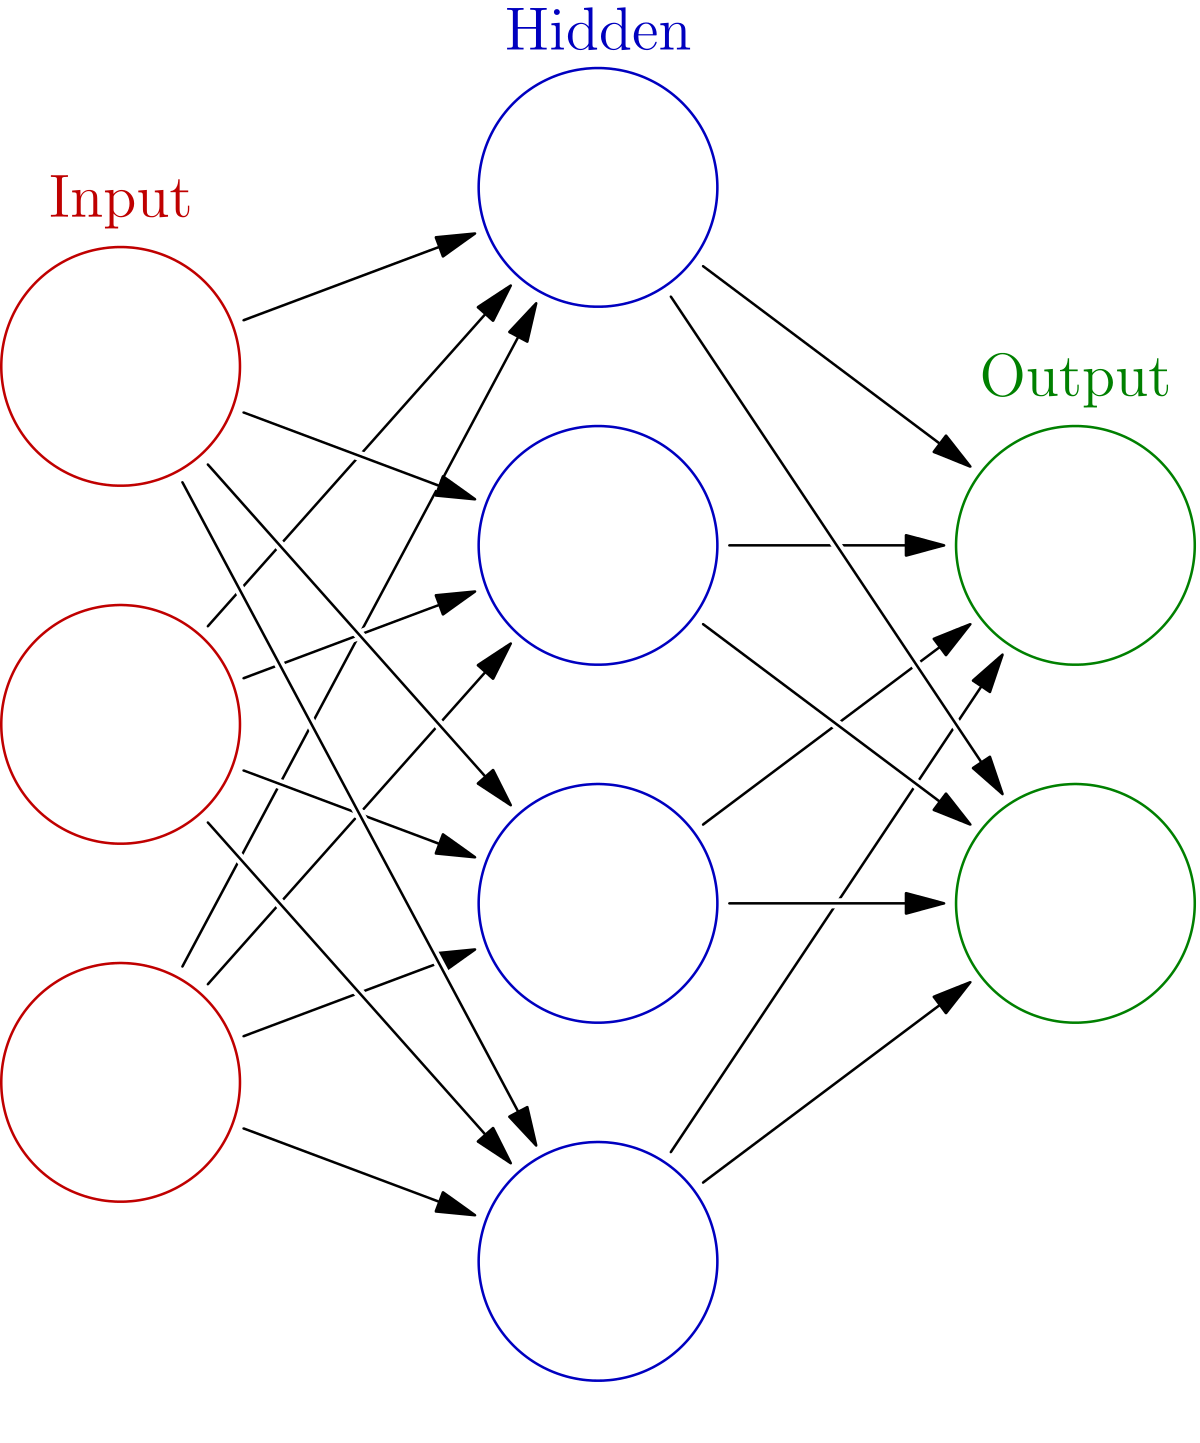
\includegraphics[width=0.35\textwidth]{Pictures/neural_network.png}
    \caption{Example of a basic feed-forward neural network}
    \label{fig:neural_network}
\end{figure}

\par
The layers in a neural network are fully connected, meaning every unit in a given layer is connected to every unit in the next layer, while each link between nodes is assigned a weight. The values of input features propagate forward through the network to the output nodes, as each unit's output is a function of the the weighted sum of inputs. We can generally define any unit's output (activation) as the following \cite{nielsenneural}:
\begin{equation*}
     a^{l}_j = \sigma\left( \sum_k w^{l}_{jk} a^{l-1}_k + b^l_j \right) 
     \label{eq:neuron_output}
\end{equation*}
where:
\begin{itemize}
    \item $a_j^l$ is the output of the $j$-th neuron in the $l$-th layer of a neural network
    \item $a_k^{l-1}$ is the output of the $k$-th neuron in the layer preceding the $l$-th layer ($l-1$)
    \item $w_{jk}^l$ is the weight of the $k$-th neuron in the previous layer ($l-1$) with respect to the $j$-th neuron in the $l$-th layer
    \item $b_j^l$ is the output of the $j$-th bias neuron in the $l$-th layer of the network
    \item $\sigma$ is an activation function
\end{itemize}

\subsection{Activation functions}
\label{sec:activation_functions}
Activation functions are used to influence the propagation of values in a neural network, as they define the outputs of nodes. Several different functions can be used and their effectiveness generally depends on properties such as differentiability and efficiency of computation, which can influence the performance of a neural network during back-propagation (process of approximating optimal weights using e.g. stochastic gradient descent). We will define two main functions that we will use later in the report: \textit{ReLU} and \textit{Softmax}.

\subsubsection{ReLU (Rectified Linear Unit)}
ReLU (Rectified Linear Unit) is a typical activation function used in deep neural networks due to its simplicity and and computational efficiency. It is defined as:
\begin{equation*}
    relu(x) = 
    \begin{cases}
        0,  & \text{if } x < 0\\
        x,  & \text{if } x \geq 0
    \end{cases}
\end{equation*}
It has been shown that, for example in convolutional neural networks, training time can improve as much as six times when using ReLU compared to previously favoured activation functions.\cite{krizhevsky2012imagenet}

\subsubsection{Softmax}
\label{sec:softmax}
The softmax function is a function that can be used in the output layers of neural networks. More specifically, it is generally used as the output activation function in multi-label classification problems in order to generate a proper probability distribution for the labels. It is defined as:
\begin{equation*}
    softmax(y_i) = \frac{e^{y_i}}{\sum_{j} e^{y_j}}
\end{equation*}
where $y$ is a vector of inputs and $y_i$ its $i$-th element

\subsection{Learning \& back-propagation}
In order to be able to classify examples using a neural network, the network has to be trained with a training data set. The goal of training a neural network is to \textit{learn} (approximate) the optimal weights the network should use in order to accurately classify data based on input. This approximation of optimal weights is facilitated by the back-propagation algorithm:
\medskip
\par
In the beginning of training, all the weights are randomly initialised. Then, for each example from the training set, the following operations are performed:
\begin{enumerate}
    \item Forward-propagate the values from the input layer ($a^1$), through hidden layers ($a^2$ to $a^{L-1}$) until the output layer values are obtained ($a^L$ where $L$ is the number of layers in the network). This can be calculated using \cref{eq:neuron_output}.
    
    \item Calculate the total error, using a cost function $C$, given each output layer value $a^L_k$ and its corresponding ground truth value (the target) $t_k$.
    
    \item Back-propagate the total error from the output layer ($L$) through hidden layers ($L-1$ until $2$) to the input layer ($1$). During back-propagation, the effect of weights on the cost $C$ is being approximated. For a given weight, this can be mathematically expressed for a node $a^l_j$ as the following partial derivative of $C$ \cite{nielsenneural}:
    \begin{equation*}
        \frac{\partial C}{\partial w^l_{jk}} = a^{l-1}_k \cdot \delta^l_j
    \end{equation*}
    where
    \begin{itemize}
        \item $C$ is the cost function
        \item $w^l_{jk}$ is the weight of the $k$-th neuron in layer $l-1$ with respect to the $j$-th neuron in layer $l$
        \item $a^{l-1}_k$ is the output (activation) of the $k$-th neuron in layer $l-1$
        \item $\delta^l_j$ is an \textit{error term} that can be derived based on the specific cost and activation functions used in the network
    \end{itemize}
    
    \item For each weight $w^l_{jk}$, update the weight according to the following assignment\cite{nielsenneural}\cite{thomas_nn_slides}:
    \begin{equation*}
        w^l_{jk} := w^l_{jk} + \eta \cdot \delta^l_j \cdot a^{l-1}_k
    \end{equation*}
    where $\eta$ is a constant factor called learning rate.
\end{enumerate}

\par
In summary, during training, batches of training examples are being fed through the network. Back-propagation is used in order to compute the gradient of the cost function $\nabla C$, based on the error between the predicted outputs and the true outputs. Then, given $\nabla C$, the network weights can be optimised for to minimise the cost, by changing them in the opposite direction of $\nabla C$. This optimisation technique, formally known as gradient descent, is what facilitates the \textit{learning} in a neural network.

\subsection{Cost function}
A cost function (also known as error or loss function) facilitates the measurement of error, given the network output and the ground truth. As described earlier, the value of the function serves as a performance metric during training and influences the weight adjustments.
\medskip
\par
\subsubsection{Cross-entropy}
The cost function that will be used in our experiments is called cross-entropy, and can be defined as \cite{nielsenneural}:
\begin{equation*}
    C = - \sum_i y_i \cdot \log(p_i)
\end{equation*}
where:
\begin{itemize}
    \item $y_i$ is the ground truth value for the $i$-th output
    \item $p_i$ is the $i$-th predicted value, corresponding to the output (activation) of the $i$-th neuron in the output layer of the network
    \item $\log$ is the natural logarithm ($\log_e$)
\end{itemize}
\medskip
\par
As mentioned earlier, our problem is that of multi-label classification and therefore our neural network output should be a probability distribution over the different classes (hence the usage of the softmax activation function in the output layer, as per \cref{sec:softmax}).
\medskip
\par
Cross-entropy is a commonly used cost function in multiple fields, when it comes to optimisation of probability distributions. In deep neural networks specifically, cross-entropy is often leveraged for the nature of its derivative, which avoids slowdown during learning.






\pagebreak
\section{Convolutional Neural Networks}

\par
Convolutional neural network (CNN) represents a deep learning model that can be used in classification problems. It can be defined as a special category of neural networks which replace the general matrix multiplication with convolutions in at least one layer of the structure.\cite{Goodfellow}
CNN is commonly used for data that follow some patterns. Complex patterns can be identified starting with simple ones in the first convolution layers. Examples of applications using CNN are: human digit recognition \cite{digits}, human activity recognition \cite{convolutional} or image classification. The input data is usually represented in the shape of a grid, but the performance is also good with 1-dimensional data.

\subsection{Convolution, mathematical concept}
\par
The intuition behind the convolutions has the bases in mathematics where the convolution of two function $f(t)$ and $g(t)$  \cite{Goodfellow} is denoted by:
\begin{equation*}
    (f*g)(t) = \int_{-\infty}^{\infty}f(\tau)g(t-\tau) d\tau
\end{equation*}

\begin{figure}[H]
    \centering
    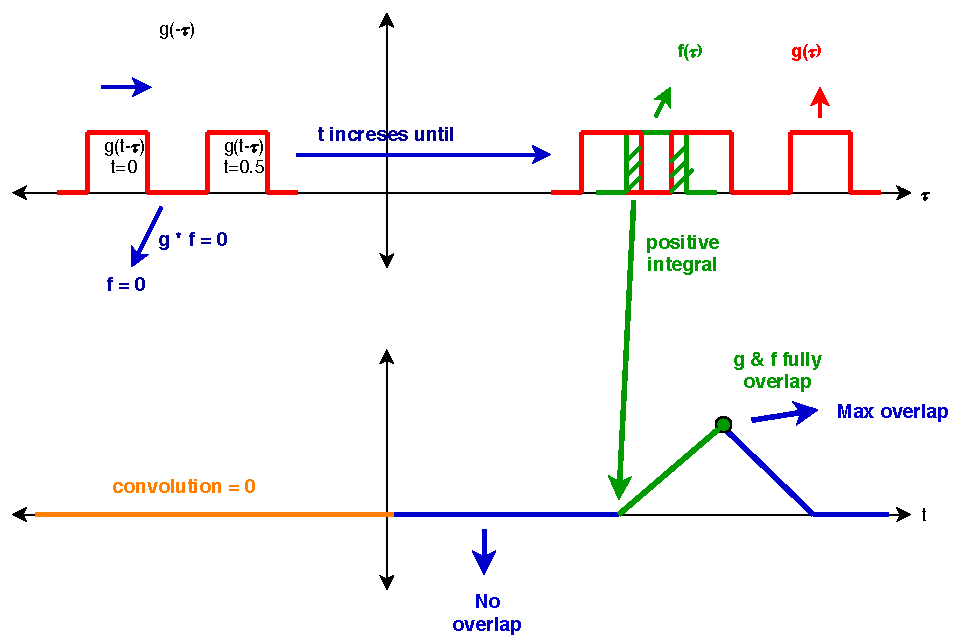
\includegraphics[width=0.8\textwidth]{convolutionMath}
    \caption{Graphical mathematical example of convolution}
    \label{fig:convolutionMath}
\end{figure}

\par
Using \cref{fig:convolutionMath} the convolution is explained as follows:
\begin{enumerate}
    \item take two functions: $f(\tau)$ and $g(\tau)$ 
	\item let then consider $g(-\tau)$, in this case f=0 and the result of $(f*g)(t) = 0$ \cref{fig:convolutionMath}
	\item sweeping $g(-\tau)$ across the domain, from $(-\infty)$ to 0, the result will remain 0 due to f = 0
	\item when $g$ starts to overlap $f$, the integral = positive value
	\item when the two functions are fully overlapped, the integral reaches the maximum value
	\item after this point g will continue to sweep across f, but the overlap zone will decrease; the value for the integral will also start to decrease until it reaches 0 again (the point where there is no more overlapping)
\end{enumerate}
 
To summarise, the convolution defined as $(f*g)(t)$ tell us the degree to which f and g overlap at t as g sweeps across the domain at t.

\subsection{CNN architecture}
\par
The CNN structure consists of an input layer, one or more hidden layers from which at least one must be a convolution layer, and the output layer. The number of layers is dependent on the problem that needs to be solved. The deeper the network is, the more complex patterns can be identified by the convolutional neural network. 
For a better understanding of a structure we will use an example of image classification.

\subsubsection{Input}
\par
The input represents data used to feed the network. It can take several shapes in terms of the size (1D, 2D, 3D). Pictures for example, can be represented by a 2D matrix where the filled pixels will have value 1 and the others 0.
\cref{fig:input} describes the transformation from an image to a 7x7 matrix input.

\begin{figure}[ht]
    \centering
    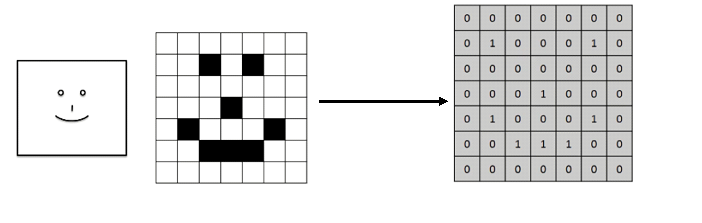
\includegraphics[width=0.9\textwidth]{CNNinput}
    \caption{Graphical example of a input}
    \label{fig:input}
\end{figure}

\subsubsection{Convolution layer}
\label{sec:convolution layer}
\par
A convolution layer has three elements: an input, one or more feature detectors( filters) and an output (feature map) which will serve as input for the next layer. Based on the number of filters defined, there can be learnt as many features as we want in a single layer.\newline
\par
A feature detector convolves the given input, searching for patterns. It has a size denoted also as kernel size. In \cref{fig:convolution} the size is set to 3x3. 

\begin{figure}[ht]
    \centering
    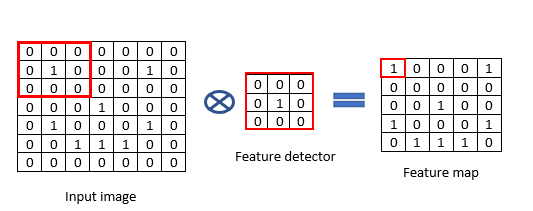
\includegraphics[width=0.9\textwidth]{convolutionLayer}
    \caption{Graphical example of a convolution layer}
    \label{fig:convolution}
\end{figure}

\begin{figure}[ht]
    \centering
    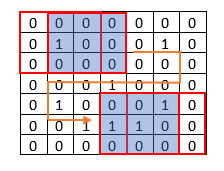
\includegraphics[width=0.5\textwidth]{filter}
    \caption{Graphical example of filter sliding}
    \label{fig:filter}
\end{figure}

\par
\cref{fig:convolution} and \cref{fig:filter} represent graphical representation of how convolution works. The steps are as follows:
\begin{enumerate}
    \item define the feature detector; let's assume that for the given example we first want to find features like an eye or the nose of the smiley face; those are represented by a single filled pixel or a value of 1 in the input matrix; the chosen filter will convolute the input to find the feature
    \item place the filter in the top-left-corner of the input
    \item compute an element-wise product between the defined filter and input matching cells
    \item store the result in the convolution layer output called feature  map as in \cref{fig:convolution}
    \item move the filter to the next column and repeat 3 and 4
    \item the filter will be sliding through all the input until it reaches the right bottom corner (\cref{fig:filter}); the filter will be moved one column at time. This movement is also called stride
    \item the feature map resulted will be the input for the next network layer
\end{enumerate}

\subsubsection{Activation layer}
\par
Another layer type that is often found in CNNs after a convolution layer is an \textit{activation} layer. The neurons of this layer use an activation function (as defined in \cref{sec:activation_functions}) in order to introduce non-linearity into the model. This process is sometimes also considered as simply part of the convolution operation.

\subsubsection{Pooling}
\label{sec:pooling layer}
\par 
The concept of pooling plays an important role in convolution neural networks, allowing the recognition of an image independently of the spatial position and also reducing the size on the input.
With our example of the smiley face the network needs to be able to correctly classify the image disregarding the position \cref{fig:positions}.

\begin{figure}[ht]
    \centering
    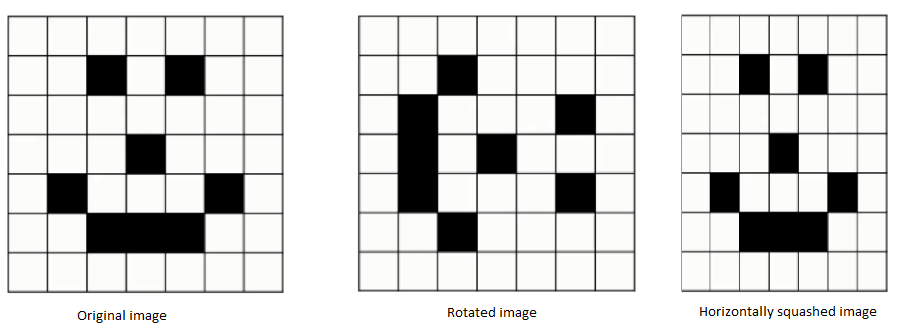
\includegraphics[width=0.8\textwidth]{smileyFacePosition}
    \caption{Graphical example of image positions}
    \label{fig:positions}
\end{figure}

\par
Pooling can be chosen differently from the existing several types according with the problem. Some of the existing types are:
\begin{itemize}
    \item max pooling
    \item min pooling
    \item mean pooling
\end{itemize}

\par
The max pooling concept it is using the feature map as input and outputs a pooled feature map. It is working based on the following steps and \cref{fig:pooling}:

\begin{figure}[H]
    \centering
    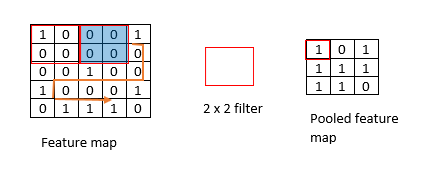
\includegraphics[width=0.8\textwidth]{maxPooling}
    \caption{Graphical example of max pooling}
    \label{fig:pooling}
\end{figure}

\begin{enumerate}
    \item define the size of the filter that will be used
    \item place the filter on top left corner of the feature map
    \item pick the maximum value from the selected region
    \item start from the top left corner and insert the selected value  
    \item define the stride value, in \cref{fig:pooling}, stride = 2
    \item move the filter along the feature map based on the stride value, and repeat 3
    \item move through the pooled feature map as the filter moves and insert the max value
\end{enumerate}
\par
The principle of min pooling or mean pooling is the same except for the way of choosing the value from the selected area. In other words, it can also be the minimum value or the mean value.\newline


\subsubsection{Fully connected layer}
\par 
A fully connected layer is a typical layer used in basic neural networks where each neuron in layer ($l$) is connected to each neuron in layer ($l-1$), as illustrated in \cref{fig:neural_network} and defined in \cref{eq:neuron_output}.

\subsubsection{Output}
\par 
The output consists of neurons where the number can vary based on the classification type (one class or multiple classes). The output of each neuron is the network's belief that the input belongs to said class. %network outputs a value interpreted as how much the network believes the input belongs to a certain class. 

\pagebreak
\section{Implementation}
\subsection{Input model}

\par
In order to utilise Convolutional Neural Network (CNN) for passenger classification, we must first decide on the nature of the input. To represent a mobile device, we can follow the steps of modelling the data defined in chapter 5. We define table $T$ to have size:

\begin{align*}
    |S| \times t_m
\end{align*}

\par
where:
\begin{itemize}
	\item $S$ is the set of sensors installed in the airport’s arrival gate
	\item $t_m$ is the maximum time stamp
\end{itemize}

\par
The size of $T$ now depends on the number of sensors that measured mobile device and number of seconds that elapsed between first and last measurement. The table size, therefore, varies for each mobile device. To use CNN, we must first reshape each mobile device table to a fixed size. We selected all 13 sensors located in the arrival gate (see \cref{fig:stat:readingspersensor}) and first 45 minutes (2700 seconds) of measurements. Figure \ref{fig:stat:timespentdistbylabel} shows that 45 minutes is a reasonable threshold - after we average the ratios per label, only $5.4\%$ of mobile devices remain in the arrival gate area longer. We define a fixed size of $13 \times 2700$ and minimum signal strength -75. We then follow the steps described in chapter 5 in order to obtain table $T$. Table $T$ now looks as following:

\begin{table}[H]
    \centering
    \begin{tabular}{|l|l|l|l|l|}
    \hline
    t    & S1  & S2  & ... & S13 \\ \hline
    0    & -70 & -75 & ... & -75 \\ \hline
    1    & -65 & -75 & ... & -70 \\ \hline
    2    & -60 & -75 & ... & -68 \\ \hline
    3    & -60 & -75 & ... & -65 \\ \hline
    4    & -50 & -75 & ... & -63 \\ \hline
    5    & -40 & -75 & ... & -60 \\ \hline
    ...  & ... & ... & ... & ... \\ \hline
    2696 & -60 & -75 & ... & -75 \\ \hline
    2697 & -75 & -75 & ... & -75 \\ \hline
    2698 & -75 & -75 & ... & -75 \\ \hline
    2699 & -75 & -75 & ... & -75 \\ \hline
    \end{tabular}
    \caption{Input table T}
\end{table}

\par
We then map each signal strength value t in the table from interval $[a, b] (a = -75, b = -3)$ to $[a', b'] (a' = 0, b' = 100)$. We do this, because we use Rectified linear unit (ReLU) as activation function in the activation layer of CNN, which returns zero on any negative input. We used the following function for mapping the signal strengths:

\begin{align*}
     f(t) =  a' +  \big( \frac{b' - a'}{b - a} \big) * (t-a), a \neq b  
\end{align*}

\par
Where:
\begin{itemize}
    \item $t$ is the signal strength
	\item $a$ is the lowest measured signal strength
	\item $b$ is the highest measured signal strength
\end{itemize}

\par
We can now apply function f to each value in the table $T$:

\begin{align*}
     T_{p_{i,j}} = f(T_{i,j})  
\end{align*}

\par
Where:
\begin{itemize}
	\item $T_{i,j}$ is the value in the  $i^{th}$  row and $j^{th}$ column of table $T$
	\item $T_{p_{i,j}}$ is the value in the $i^{th}$ row and $j^{th}$ column of table $T_p$
\end{itemize}

\par
The table $T_p$ can be represented as a matrix $P$, which we can use as an input for the convolutional neural network:

\begin{align*}
        P = 
        \begin{bmatrix}
            6.94     & 0        & \cdots & 0        \\
            13.89    & 0        & \cdots & 6.94     \\
            20.83    & 0        & \cdots & 9.72     \\
            20.83    & 0        & \cdots & 13.89    \\
            \vdots   & \vdots   & \ddots & \vdots   \\
            20.83    & 0        & \cdots & 0        \\
            0        & 0        & \cdots & 0        \\
            0        & 0        & \cdots & 0        
        \end{bmatrix}
\end{align*}

\subsection{Design}
\label{sec:cnn:design}

\par 
The Convolutional neural network consists of convolutional, pooling, activation and fully connected layers. Fig \ref{fig:cnn:design1} shows how the input matrix $P$ flows through convolutional, pooling and activation layers. The output of the last activation layer is then flattened into a layer of neurons, as shown on Fig \ref{fig:cnn:design2}.

\begin{figure}[H]
    \centering
    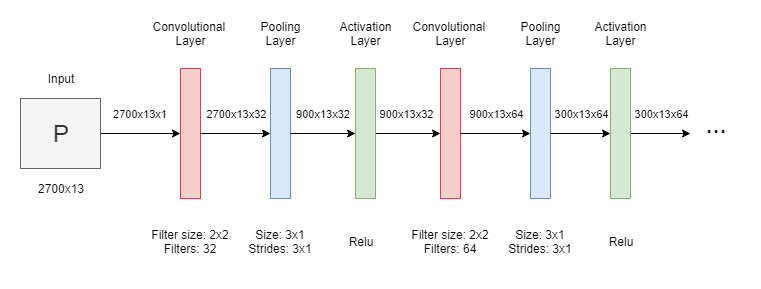
\includegraphics[width=.9\textwidth]{Pictures/Cnn_design1.png}
    \caption{CNN Flow chart 1}
    \label{fig:cnn:design1}
\end{figure}

\begin{figure}[H]
    \centering
    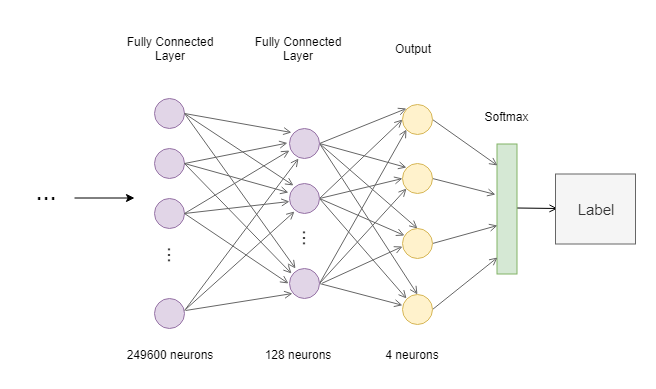
\includegraphics[width=.9\textwidth]{Pictures/Cnn_design2.png}
    \caption{CNN Flow chart 2}
    \label{fig:cnn:design2}
\end{figure}

\par
The first convolutional layer takes a single matrix $P$ as an input. It creates 32 filters of size $2 \times 2$ and each filter convolves over $P$ (as described in section \ref{sec:convolution layer}) without skipping any rows and columns. Each filter outputs its own convoluted matrix, therefore the output of the first convolutional layer has 32 channels. The dimensions of the all output matrices remain the same as dimensions of $P$. The layer output can defined as follows:

\begin{align*}
     P_{1} = 2700 \times 13 \times 32 
\end{align*}

\par
The first pooling layer takes the output $P_{1}$ and down-samples it with a $3 \times 1$ filter (as described in section \ref{sec:pooling layer}). This filter is applied to every sub-region of every input matrix. The output of this layer can be defined as follows:

\begin{align*}
     P_{2} = 900 \times 13 \times 32 
\end{align*}

\par
The output $P_{2}$ is then passed through an activation layer. This layer uses the Rectified linear unit activation function, which ensures that any negative value in the input matrices is set to 0. The dimensions of the output do not change:

\begin{align*}
     P_{3} = P_{2} 
\end{align*}

\par 
The second convolutional layer takes an input P3 and creates 64 filters of size $2 \times 2$. The output of this layer has 64 channels and dimensionality of each input matrix remains the same. The output of this layer can be defined as follows:

\begin{align*}
     P_{4} = 900 \times 13 \times 64
\end{align*}

\par
The second pooling takes and input P4 and down-samples it with a $3 \times 3$ filter. The output of this layer can be defined as follows:

\begin{align*}
     P_{5} = 300 \times 13 \times 64
\end{align*}

\par
As before, the next activation layer applies the Rectified linear unit activation function. The dimensions of the output do not change:

\begin{align*}
     P_{6} = P_{5} 
\end{align*}

\par 
The output $P_{6}$ is then flattened into one layer of neurons. The number of neurons of the first fully connected layer can be calculated by multiplying all dimensions of the output  $P_{6}$, which is equal to 249600 neurons. These neurons are then connected to the second fully connected layer, which contains 128 neurons. The output layer then estimates how likely it is that the input image belongs to each of the 4 labels – manual, staff, no queue and privium.

\par 
To normalise the output values, we use the softmax function, which ensures that each label value is between 0 and 1, and that all 4 labels sum to 1, representing the probability distribution of the labels. The argmax function then selects the largest probability, which corresponds to the predicted label.

\subsection{Evaluation}

\par 
We selected all mobile addresses from the seven days of data measured from $6^{th}$ to $12^{th}$ September 2018. We used 13530 unique addresses distributed as follows:

\begin{itemize}
	\item manual - 3574 addresses
	\item staff - 8045 addresses
	\item no-q - 1633 addresses
	\item privium - 278 addresses
\end{itemize}

\par
The CNN model was configured according to the network design in \cref{sec:cnn:design}, alongside with the following hyper-parameters: 
\begin{itemize}
	\item number of training examples - 9065
	\item number of testing examples - 4465
	\item learning rate - 0.0001 ($10^{-4}$)
	\item batch size - 16
	\item number of optimisation iterations - 1000
	\item number of epochs - 1
\end{itemize}

\par
The CNN model was trained on two thirds of addresses, such that two thirds of addresses were randomly selected from each label. Testing set consisted of the remaining third, distributed as follows:

\begin{itemize}
	\item manual - 1179 addresses
	\item staff - 2655 addresses
	\item no-q - 539 addresses
	\item privium - 92 addresses
\end{itemize}

\par
The following confusion matrix breaks down the performance of this model:

\begin{figure}[H]
    \centering
    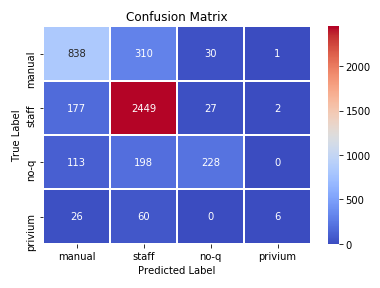
\includegraphics[width=.5\textwidth]{Pictures/Cnn_cm2.png}
    \caption{CNN results (Confusion matrix)}
    \label{fig:cnn:cm}
\end{figure}

\par
As described in \ref{section:performance_metrics}, the following is the performance summary of CNN derived from the confusion matrix above:

\begin{table}[H]
    \centering
    \begin{tabular}{|l|c|c|c|}
    \hline
                            & \textbf{Precision} & \textbf{Recall} & \textbf{Examples} \\ \hline
    \textbf{manual}         & 0.73               & 0.71            & 1179               \\ \hline
    \textbf{staff}          & 0.81               & 0.92            & 2655               \\ \hline
    \textbf{no-q}           & 0.80               & 0.42            & 539                \\ \hline
    \textbf{privium}        & 0.67               & 0.07            & 92                 \\ \hline
    \textbf{Average/ Total} & 0.7525             & 0.53           & 4465              \\ \hline
    \textbf{Accuracy}       & \multicolumn{3}{c|}{78.9}                                \\ \hline
    \end{tabular}
    \caption{Performance summary for CNN}
\end{table}

\pagebreak
\section{Interpretation and Conclusion}

\par
The overall accuracy of this model was considerably higher compared to other previously utilised models. The model itself performed the worst when it comes to classification of privium and no-q passengers. This could be due to small number of examples in the data-set for both labels. On the other hand we can conclude that the model performs a lot better with classification of manual passengers and staff members, which are the most common types of mobile devices detected at the arrival gate. 